\subparagraph{Задание 4.8}

\textbf{Условие}:
Выполнить программу (Goto cursor - клавиша \textbf{F4}) до места начала цикла. 

\textbf{Решение}:

Есть стрелка.
Рисунок~\ref{fig:task_4_8__1} (стр.~\pageref{fig:task_4_8__1}).
Нижние подчеркивание двигается.
Рисунок~\ref{fig:task_4_8__2} (стр.~\pageref{fig:task_4_8__2}).
Жмем \textbf{F4}. Стрелка встала на нижнее подчеркивание.
Рисунок~\ref{fig:task_4_8__3} (стр.~\pageref{fig:task_4_8__3}).

\begin{figure}[!htp]
    \centering
    \begin{minipage}{0.32\textwidth}
        \centering
        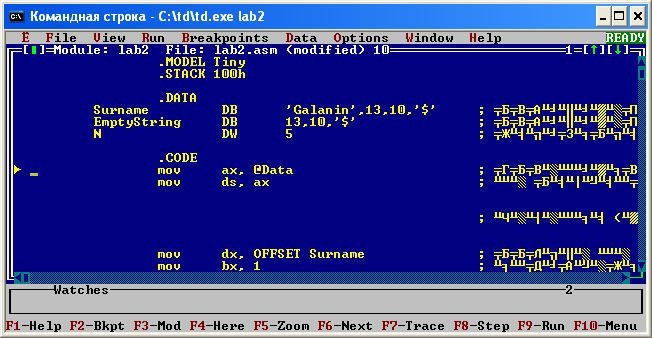
\includegraphics[width=.99\linewidth]
            {../_INCLUDES/task-4-8/1.png}
        \caption{1) Начальное состояние}
        \label{fig:task_4_8__1}
    \end{minipage}
    \begin {minipage}{0.32\textwidth}
        \centering
        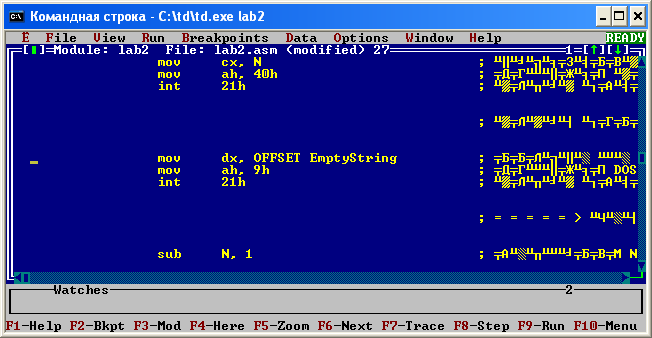
\includegraphics[width=.99\linewidth]
            {../_INCLUDES/task-4-8/2.png}
        \caption{2) Поставили метку стрелками \textbf{вверх}-\textbf{вниз}}
        \label{fig:task_4_8__2}
    \end{minipage}
    \begin {minipage}{0.32\textwidth}
        \centering
        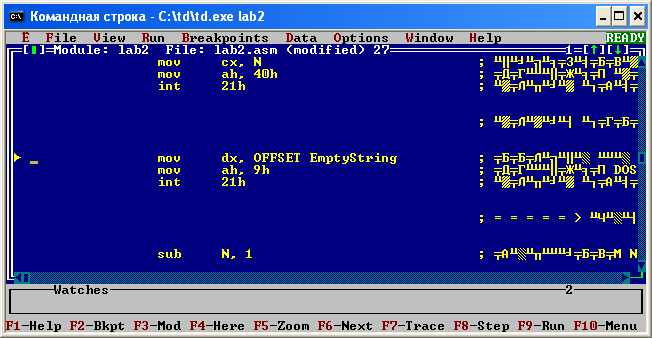
\includegraphics[width=.99\linewidth]
            {../_INCLUDES/task-4-8/3.png}
        \caption{3) Перешли к метке клавишей \textbf{F4}}
        \label{fig:task_4_8__3}
    \end{minipage}
\end{figure}
